\documentclass{article}

% Math packages
\usepackage{amsthm, amssymb}

% Margins settings
\usepackage[margin=1.2in]{geometry}

% Bracket notation (quantum computing/information)
\usepackage{tikz}
\usetikzlibrary{quantikz}
\usepackage{braket}

% Spacing
\usepackage{parskip}
\usepackage{centernot}

% Required for inserting images
\usepackage{graphicx}
\graphicspath{{./Figures/}}

% Hyperlinks
\usepackage[colorlinks=true, allcolors=blue]{hyperref}

% Header
\usepackage{fancyhdr}
\pagestyle{fancy}
\lhead{October 28th, 2024}
\chead{Optimization for Data Science}
\rhead{University of Waterloo}

% Custom commands
\newcommand{\R}{\mathbb{R}}
\newcommand{\E}{\text{E}}
\newcommand{\ds}{\displaystyle}
\newcommand{\indep}{\perp\!\!\!\perp}

\setlength\parindent{0pt}

\title{CO 673/CS 794 - Optimization for Data Science\\Lecture 14 Notes}
\author{University of Waterloo}
\date{October 28th, 2024, 11h30-12h50 in MC 2054}

\begin{document}

\maketitle

\section{Administration}

\begin{itemize}
    \item Problem set 4 due Friday at 19h00
\end{itemize}

\section{Suppose-Vector Machines}

Support-vector machine solves the following problem:

Given linearly separable data points, find the separatore farthest from the data points.

From the previous lecture: SVM-3:
\[
    \max_{\vec{x},\, \xi,\, \vec{t}}\left(\min_{j \in \{1,\, \ldots,\, N\}}\left(t_j\right)\right)
\]
such that
\[
    \|\vec{x}\| \leq 1 \quad \wedge \quad \begin{cases}
        \vec{a}_j^\top \vec{x} + \xi = t_j, & y_j = 1 \\
        \vec{a}_j^\top \vec{x} + \xi = -t_j, & y_j = -1
    \end{cases}
\]

\begin{center}
    \includegraphics*[scale=0.13]{hyperplane.JPG}

    \small Examples of hyperplane
\end{center}


Problem: Non-smooth. We introduce  $\widetilde{t} = \min_j(\{t_j\})$. SVM-4:
\[
    \max_{\vec{x},\, \xi,\, \widetilde{t}}
\]
such that
\[
    \|\vec{x}\| \leq 1 \quad \wedge \quad \begin{cases}
        \vec{a}_j^\top \vec{x} + \xi \geq \widetilde{t}, & y_j = 1 \\
        \vec{a}_j^\top \vec{x} + \xi \leq -\widetilde{t}_j, & y_j = -1
    \end{cases}
\]

If for a feasible solution of SVM-4. We define:
\[
    t_j =  \begin{cases}
        \vec{a}_j^\top \vec{x} + \xi, & y_j = 1 \\
        -\left(\vec{a}_j^\top \vec{x} + \xi\right), & y_j = -1
    \end{cases}
\]
These constraints imply that $\forall j$, $t_j \geq \widetilde{t} \implies \min_j(\{t_j\}) \geq \widetilde{t}$. This must be satisfeid as the equality holds at the optimizer.

We define $\vec{x}' = \frac{\vec{x}}{\widetilde{t}}$ and $\xi' = \frac{\xi}{\widetilde{t}}$, where $\widetilde{t} > 0$ at the optimizer.

We divide the inequality constraints by $\widetilde{t}$. SVM-5:
\[
    \max\left(\left\{\widetilde{t}\right\}\right)
\]
such that
\[
    \left\|\widetilde{t}\vec{x}'\right\| \leq 1 \quad \wedge \quad \begin{cases}
        \vec{a}_j^\top \vec{x}' + \xi' \geq 1, & y_j = 1 \\
        \vec{a}_j^\top \vec{x}' + \xi' \leq -1, & y_j = -1
    \end{cases} \tag{$\dag$}
\]
We observe that the problem $ \max\left(\left\{\widetilde{t}\right\}\right)$ such that $(\dag)$ is equivalent to the problem $\min\left(\left\{\|\vec{x}'\right\}\right)$ such that $(\dag)$. This is because, at the optimizer, for SVM-5, we always select $\widetilde{t} = \frac{1}{\|\vec{x}'\|}$ which leads to SVM-6 (we drop the apostraphes).

SVM-6:
\[
    \min\left(\left\{\|\vec{x}\|\right\}\right)
\]
such that
\[
    \begin{cases}
        \vec{a}_j^\top \vec{x} + \xi \geq 1, & y_j = 1 \\
        \vec{a}_j^\top \vec{x} + \xi \leq -1, & y_j = -1
    \end{cases}
\]
this is called "hard-margin SVM".

What if the data points are not affinely separable?

SVM-7 (soft-margin SVM):
\[
    \min\left(\left\{\|\vec{x}\|^2 + \gamma \sum_j s_j\right\}\right)
\]
such that
\[
    \forall j,\, s_j \geq 0 \quad \wedge \quad \begin{cases}
        \vec{a}_j^\top \vec{x} + \xi \geq 1 - s_j, & y_j = 1 \\
        \vec{a}_j^\top \vec{x} + \xi \leq -1 + s_j, & y_j = -1
    \end{cases}
\]
where $s_j = 0 \implies$ point properly classified, and $\gamma > 0$ is a tuning parameter. We can produce an equivalent, unconstrained, non-smooth problem:

Given $\vec{x}$ and $\xi$, find the optimal $s_j$'s in closed form.

For $y_j = 1$, we choose
\[
    s_j = \begin{cases}
        0, & \vec{a}_j^\top\vec{x} + \xi \geq 1 \\
        1 - \left(\vec{a}_j^\top \vec{x} + \xi\right), & \vec{a}_j^\top\vec{x} + \xi \leq 1
    \end{cases} = \varphi\left(\vec{a}_j^\top\vec{x} + \xi\right)
\]
where $\varphi(t) = \max(\{0,\, 1 - t\})$
\begin{center}
    \includegraphics*[scale=0.4]{phi.png}
\end{center}
For $y_j = -1$, we choose
\[
    s_j = \begin{cases}
        0, & \vec{a}_j^\top\vec{x} + \xi \leq -1 \\
        1 + \left(\vec{a}_j^\top \vec{x} + \xi\right), & \vec{a}_j^\top\vec{x} + \xi \geq -1
    \end{cases} = \widetilde{\varphi}\left(\vec{a}_j^\top\vec{x} + \xi\right)
\]
where $\varphi(t) = \max(\{0,\, 1 - t\})$
\begin{center}
    \includegraphics*[scale=0.4]{phi_tilde.png}
\end{center}
which yields SVM-8:
\[
    \min_{\vec{x},\, \xi}\left(\left\{\|\vec{x}\|^2 + \gamma \sum_{j : y_j = 1} \varphi\left(\vec{a}_j^\top\vec{x} + \xi\right) + \gamma \sum_{j : y_j = -1} \widetilde{\varphi}\left(\vec{a}_j^\top\vec{x} + \xi\right)\right\}\right)
\]
which is convex, unconstrained, and non-smooth. This $\varphi$ (as well as $\widetilde{\varphi}$) is called the \textbf{hinge loss}.

Note that the above is quite similar to logistic regression with $\ell_2$ regularization. The differences are:
\begin{itemize}
    \item the position of parameter $\gamma$,
    \item hinge loss vs logistic loss,
    \item SVM-8 does not regularize $\xi$
\end{itemize}
There is a big extension of SVM to kernel machines. We consider constrained optimization:
\[
    \min\left(\left\{f(\vec{x})\right\}\right) \quad \text{s.t.} \quad \vec{x} \in \Omega \subseteq \R^n
\]
where $\Omega$ is closed and convex.

The normal cone, $\text{N}_{\Omega}(\vec{x})$ at $\vec{x} \in \Omega$ is defined as:
\[
    \text{N}_{\Omega}(\vec{x}) = \left\{\vec{v} \in \R^n : \forall \vec{y} \in \Omega,\, \vec{v}^\top(\vec{y} - \vec{x}) \leq 0\right\}
\]
\begin{center}
    \includegraphics*[scale=0.12]{normal_cone.JPG}
\end{center}
A closed and convex cone, $C$ is defined by
\begin{enumerate}
    \item $\vec{0} \in C$,
    \item $\forall \lambda \geq 0,\, \vec{x} \in C \implies \lambda\vec{x} \in C$,
    \item $\vec{x},\, \vec{y} \in C \implies \vec{x} + \vec{y} \in C$
\end{enumerate}

\textbf{Theorem 7.2}

Suppose that $\Omega \subseteq \R^n$ is closed, non-empty, and convex. Also suppose that $f\colon \R^n \to \R \cup \{\infty\}$ is convex, differentiable, and $\Omega \in \text{dom}(f)^\circ$. Then, $\vec{x}^*$ is a minimizer of $f$ over $\Omega$ if, and only if,
\[
    \vec{x}^* \in \Omega \wedge -\nabla f(\vec{x}^*) \in \text{N}_{\Omega}(\vec{x}^*)
\]

\begin{center}
    \includegraphics*[scale=0.08]{minimizer.JPG}
\end{center}

\begin{proof}
    $(\impliedby)$:

    Let $\vec{z} \in \Omega$. Then, by the subgradient inequality,
    \[
        f(\vec{z}) \leq f(\vec{x}^*) + \underbrace{\nabla f(\vec{x}^*)^\top(\vec{z} - \vec{x}^*)}_{\geq\, 0\, (**)}
    \]
    (**) since $-\nabla f(\vec{x}^*) \in \text{N}_{\Omega}(\vec{x}^*)$ and $\vec{z} \in \Omega$

    $(\implies)$:

    $\forall \vec{z} \in \Omega$, $\forall \alpha \in [0;\; 1]$, we have that
    \begin{align*}
        f(\vec{x}^*) &\leq f((1 - \alpha)\vec{x}^* + \alpha\vec{z}) \\
        &= f(\vec{x}^* + \alpha(\vec{z} - \vec{x}^*)) \\
        &\overset{\text{def}}{=} f(\vec{x}^*) + \alpha \nabla f(\vec{x}^*)^\top(\vec{z} - \vec{x}^*) + \varphi_{\vec{x}^*}(\alpha(\vec{z} - \vec{x}^*))
    \end{align*}
    We subtract $f(\vec{x}^*)$; we assume that $\alpha > 0$ and divide by $\alpha$. We take the limit as $\alpha \to 0$:
    \begin{align*}
        &\implies \nabla f(\vec{x}^*)^\top(\vec{z} - \vec{x}^*) \geq 0 \implies -\nabla f(\vec{x}^*) \in \text{N}_{\Omega}(\vec{x}^*)
    \end{align*}
\end{proof}

How do we write the normal cone of a region specified by constraints?

\textbf{Theorem (8.15).}

Suppose that $\left\{\Omega_k\right\}_{k = 1}^{k = m} \subset \mathcal{P}(\R^n)$, where $\forall k$, $\Omega_k$ is closed and convex. We define $\Omega$ as follows:
\[
    \Omega = \bigcap_{k = 1}^{k = m} \Omega_k
\]
then $\Omega$ is also closed and convex, and $\forall \vec{x} \in \Omega$,
\[
    \sum_{k = 1}^{k = m} \text{N}_{\Omega_k}(\vec{x}) \subseteq \text{N}_{\Omega}(\vec{x}) \tag{*}
\]
where the sum above is the Minkowsky sum defined as follows: $\forall A,\, B \subseteq \R^n$,
\[
    A + B := \left\{a + b : a \in A,\, b \in B\right\}
\]
\begin{proof}
    For $k = 1 : m$, let $\vec{v}_k \in \Omega_k$. Let $\vec{v} = \sum_{k = 1}^{k = m} \vec{v}_k$. Let $\vec{z} \in \Omega$. By the definition of $\text{N}_{\Omega_k}$, $\vec{v}_k^\top(\vec{z} - \vec{x}) \leq 0$. Thus,
    \[
        \vec{v}^\top(\vec{z} - \vec{x}) \leq 0 \implies \vec{v} \in \text{N}_{\Omega}(\vec{x})
    \]
\end{proof}
Constrain qualification: Assumption imposed on $\Omega_k$'s to ensure (*).

Fact: If $\forall k \in \{1,\, \ldots,\, m\}$, $\Omega_k$ is a polyhedron, then $\forall \vec{x} \in \R^n$, (*) holds.

Fact: If $\bigcap_{k = 1}^{k = m} \Omega_k^\circ = \varnothing$, then $\forall \vec{x} \in \R^n$, (*) holds.

Example of when (*) fails:

Let $n = 2$, $m = 2$, $\Omega_1 = \{\vec{x} \in \R^2 : x_2 \leq 0\}$, and $\Omega_1 = \{\vec{x} \in \R^2 : x_2 \geq x_1^2\}$:

\begin{center}
    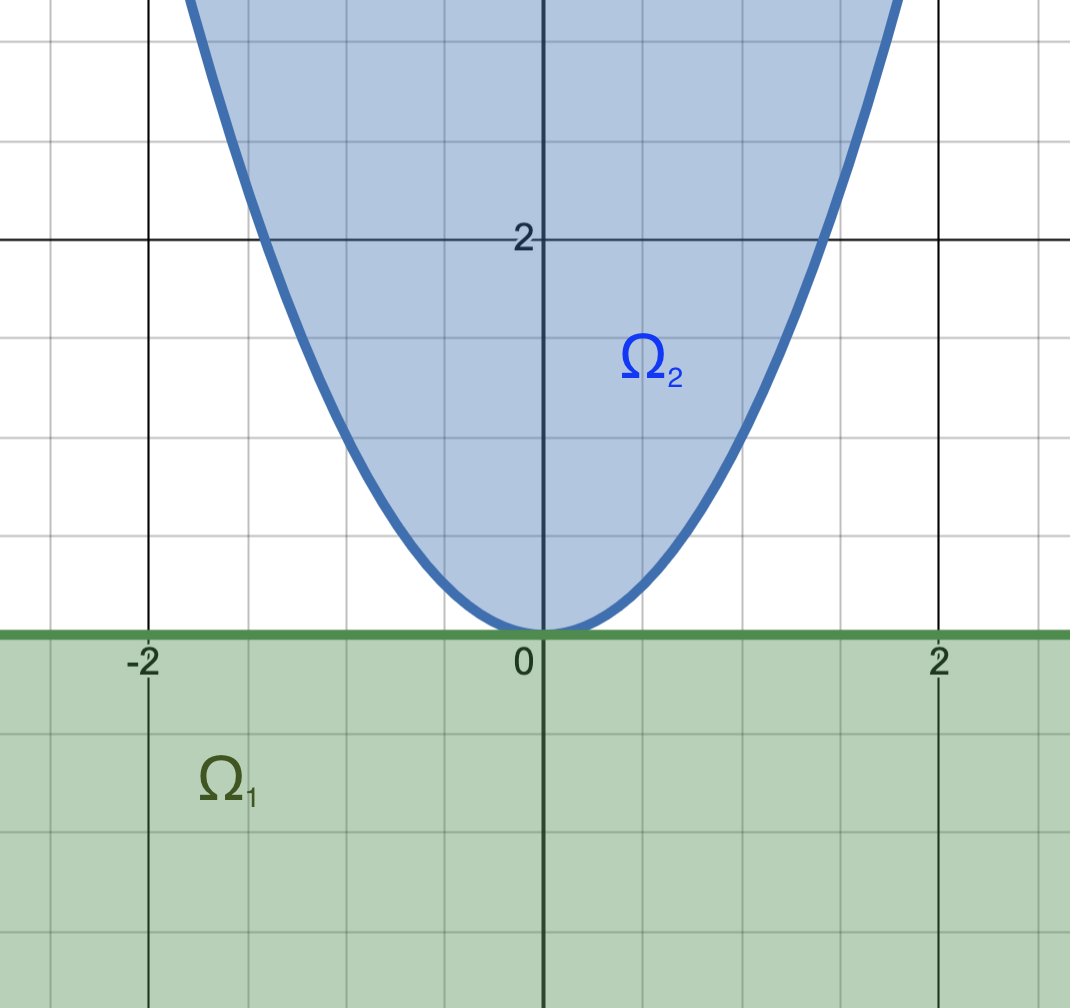
\includegraphics[scale=0.5]{Omegas.png}
\end{center}

We have
\[
    \text{N}_{\Omega_1}\left(\vec{0}\right) = \left\{\begin{bmatrix}
    0 \\ x_2 \end{bmatrix} : x_2 \geq 0\right\} \quad  \text{N}_{\Omega_2}\left(\vec{0}\right) = \left\{\begin{bmatrix}
    0 \\ x_2 \end{bmatrix} : x_2 \leq 0\right\}
\]
Hence,
\[
    \Omega = \Omega_1 \cap \Omega_2 = \left\{\vec{0}\right\}
\]
Thus,
\[
    \text{N}_{\Omega}\left(\vec{0}\right) = \R^2 \quad \text{since} \quad \forall \vec{v} \in \R^2,\, \vec{v}^\top\left(\vec{0} - \vec{0}\right) \leq 0.
\]
However,
\[
    \text{N}_{\Omega_1}\left(\vec{0}\right) + \text{N}_{\Omega_2}\left(\vec{0}\right) = \left\{\begin{bmatrix}
        0 \\ x_2 \end{bmatrix} : x_2 \in \R^2\right\}
\]

\end{document}
